\ac{sturesy} ist der Name einer freien Software, die im Rahmen der Bachelorarbeit von Wolf Posdorfer im Jahr 2012 an der Universität Hamburg entstanden ist\cite{sturesy}. Der Name StuReSy ist ein Akronym für „\textbf{Stu}dent \textbf{Re}sponse \textbf{Sy}stem“. StuReSy wurde erfolgreich und viele Jahre an der Universität Hamburg und HAW Hamburg eingesetzt. Die Qualität und der Umfang der Software sind für das Resultat einer Bachelorarbeit beeindruckend.

StuReSy besteht aus zwei Komponenten:
\begin{itemize}
    \item \textbf{Server}: In PHP geschrieben, stellt gleichzeitig die Client-Benutzeroberfläche für die Abstimmungs-Teilenehmer als auch eine Administrations-Oberfläche bereit. Benötigt eine relationale SQL-Datenbank.
    \item \textbf{Editor}: In Java geschrieben, verbindet sich mit dem Server. Um Fragen zu erstellen, zu bearbeiten und Umfragen zu starten.
\end{itemize}

Der StuReSy-Editor verfügt über folgende Hauptfunktionen bzw. Programmteile:
\begin{itemize}
    \item \textbf{Abstimmung}: Durchführung einer Umfrage
    \item \textbf{Fragen-Editor}: Erstellung und Bearbeitung von Fragesätzen.
    \item \textbf{Abstimmungs-Analyse}: Auswerten von Abstimmungs-Ergebnissen im Nachhinein.
\end{itemize}

\begin{figure}[H]
    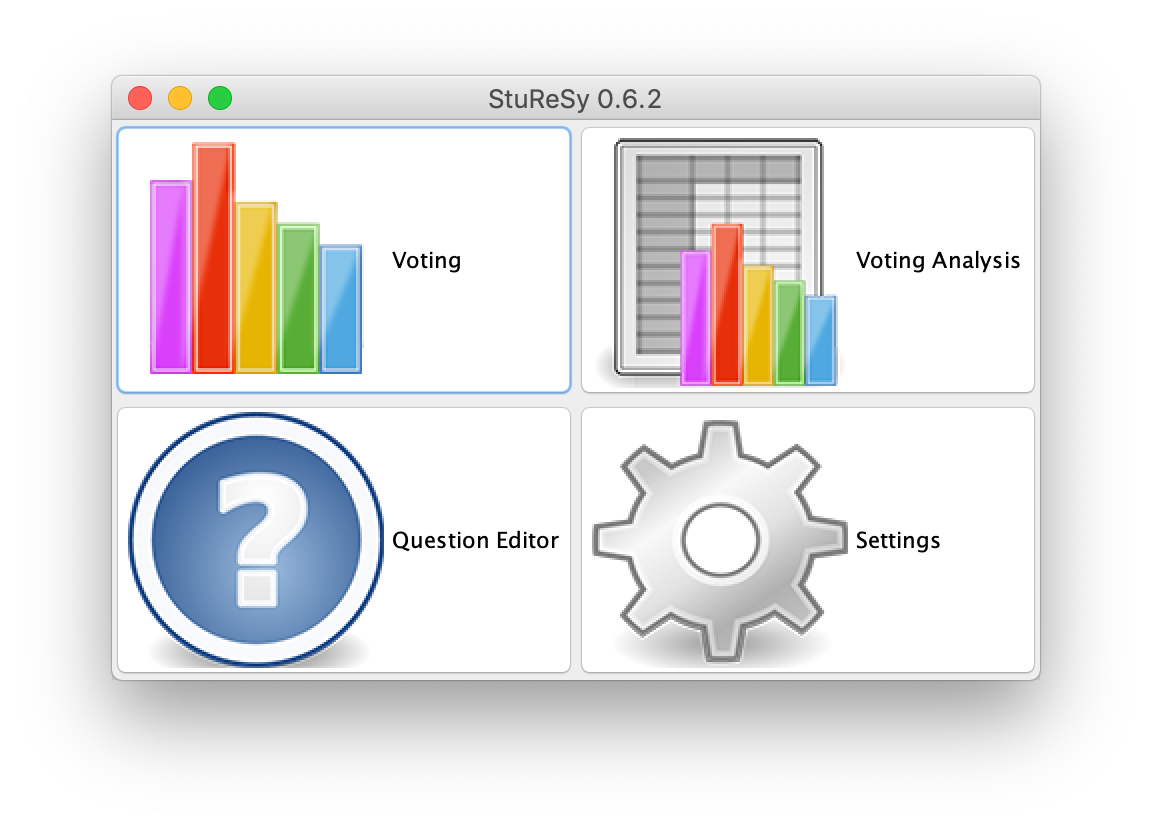
\includegraphics[width=10cm]{chapter/bewertung/bilder/StuReSy_Hauptmenue.png}
    \centering
    \caption{Hauptmenü der StuReSy-Editor-Komponente.}
    \label{abb:sturesy_hauptmenue}
\end{figure}


Auch wenn StuReSy erfolgreich im Hochschulbetrieb verwendet wurde, so gibt es trotzdem einige konzeptionelle Nachteile:
\begin{itemize}
    \item \textbf{Software-Download und Java notwendig}: Um StuReSy administrativ einsetzen zu können, muss zwangsläufig Software heruntergeladen werden und eine Java-Installation muss auf dem jeweiligen System vorhanden sein. Administrativer Zugang vom Tablet oder Smartphone aus ist damit fast nicht möglich.
    \item \textbf{Server notwendig}: Um StuReSy betreiben zu können, wird zwingend eine Instanz des StuReSy-Servers benötigt. Diese muss von der jeweiligen Institution oder einem Dozenten aufgesetzt und gewartet werden.
    \item \textbf{Kompliziertes System von Tokens und Lecture-IDs}: Um eine Abstimmung in StuReSy durchzuführen, muss zunächst eine Lecture-ID in der Server-Admin-Oberfläche eingerichtet werden. Anschließend muss ein generierter Token in den Java-Client übertragen werden. Diese Vorgehensweise erscheint unnötig kompliziert und sorgt dafür, dass nur der Administrator der Server-Komponente neue Lecture-IDs einrichten kann. Ein niedrigschwelliger Einsatz (zum Beispiel für Studenten untereinander, oder für Dozenten zum Ausprobieren) wird damit ausgeschlossen.
\end{itemize}

Neben den konzeptionellen Problemen gibt es auch Probleme mit der Implementierung von StuReSy, die sich gerade im Bereich der Programmierlehre bemerkbar machen, denn dort beinhalten die Fragetexte oft Quelltext-Ausschnitte:
\begin{itemize}
\item \textbf{Mangelnde Formatierungsmöglichkeiten}: Die Darstellung von Quelltexten in StuReSy ist schwierig. Obwohl die Formatierung von Fragen mittels HTML unterstützt wird, ist es nicht leicht, hier ordentliche Ergebnisse zu erzielen, ohne manuell HTML-Code zu editieren. Beispiele dieser Probleme sind in den Abbildungen \ref{abb:sturesy_problem_1}, \ref{abb:sturesy_problem_2} und \ref{abb:sturesy_problem_3} dargestellt.
\end{itemize}

\begin{figure}[H]
    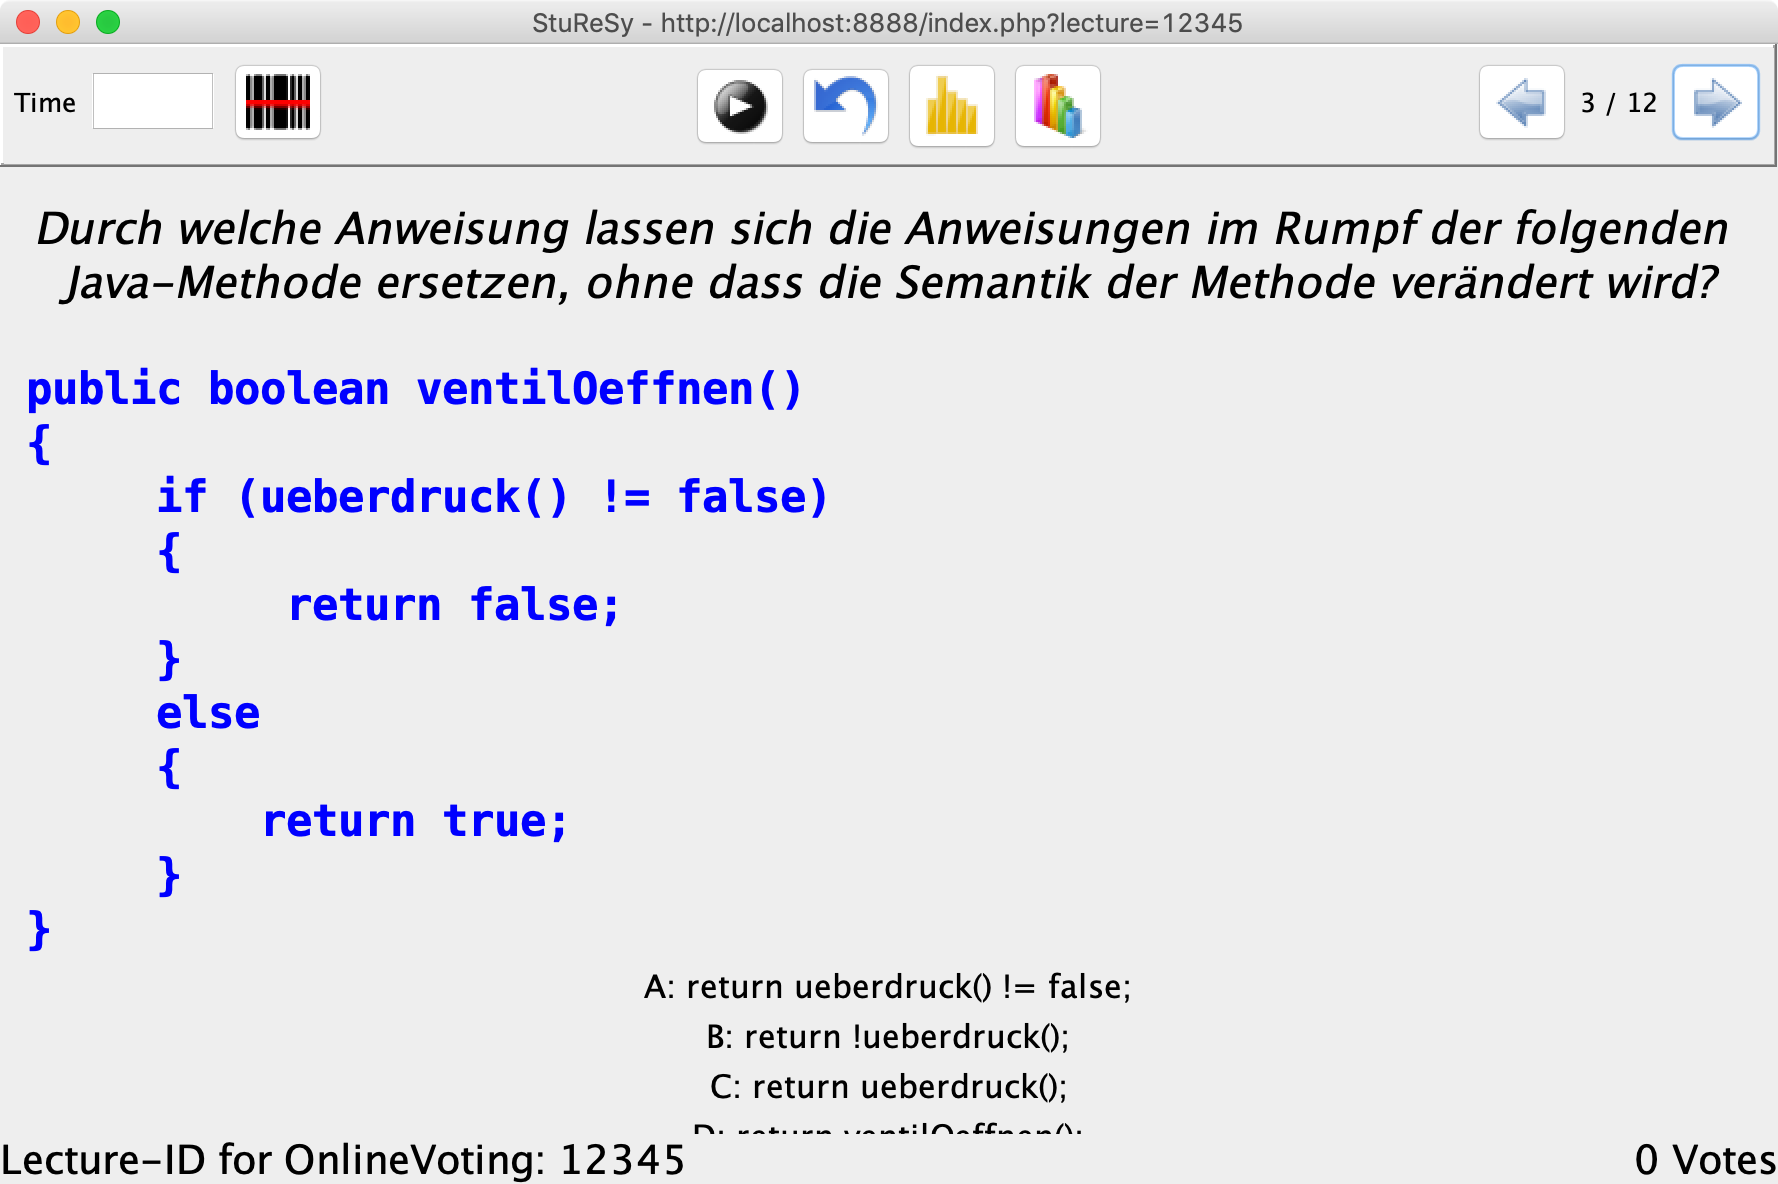
\includegraphics[width=12cm]{chapter/bewertung/bilder/StuReSy_Problem_2.png}
    \centering
    \caption{Probleme bei der Darstellung von Quelltexten: Im Gegensatz zur Fragestellung wirkt der linksbündige Quelltext deplatziert. Eine Antwort-Möglichkeit wird vom zu kleinen Fenster verdeckt. Syntax-Highlighting ist nicht vorhanden.}
    \label{abb:sturesy_problem_1}
\end{figure}

\begin{figure}[H]
    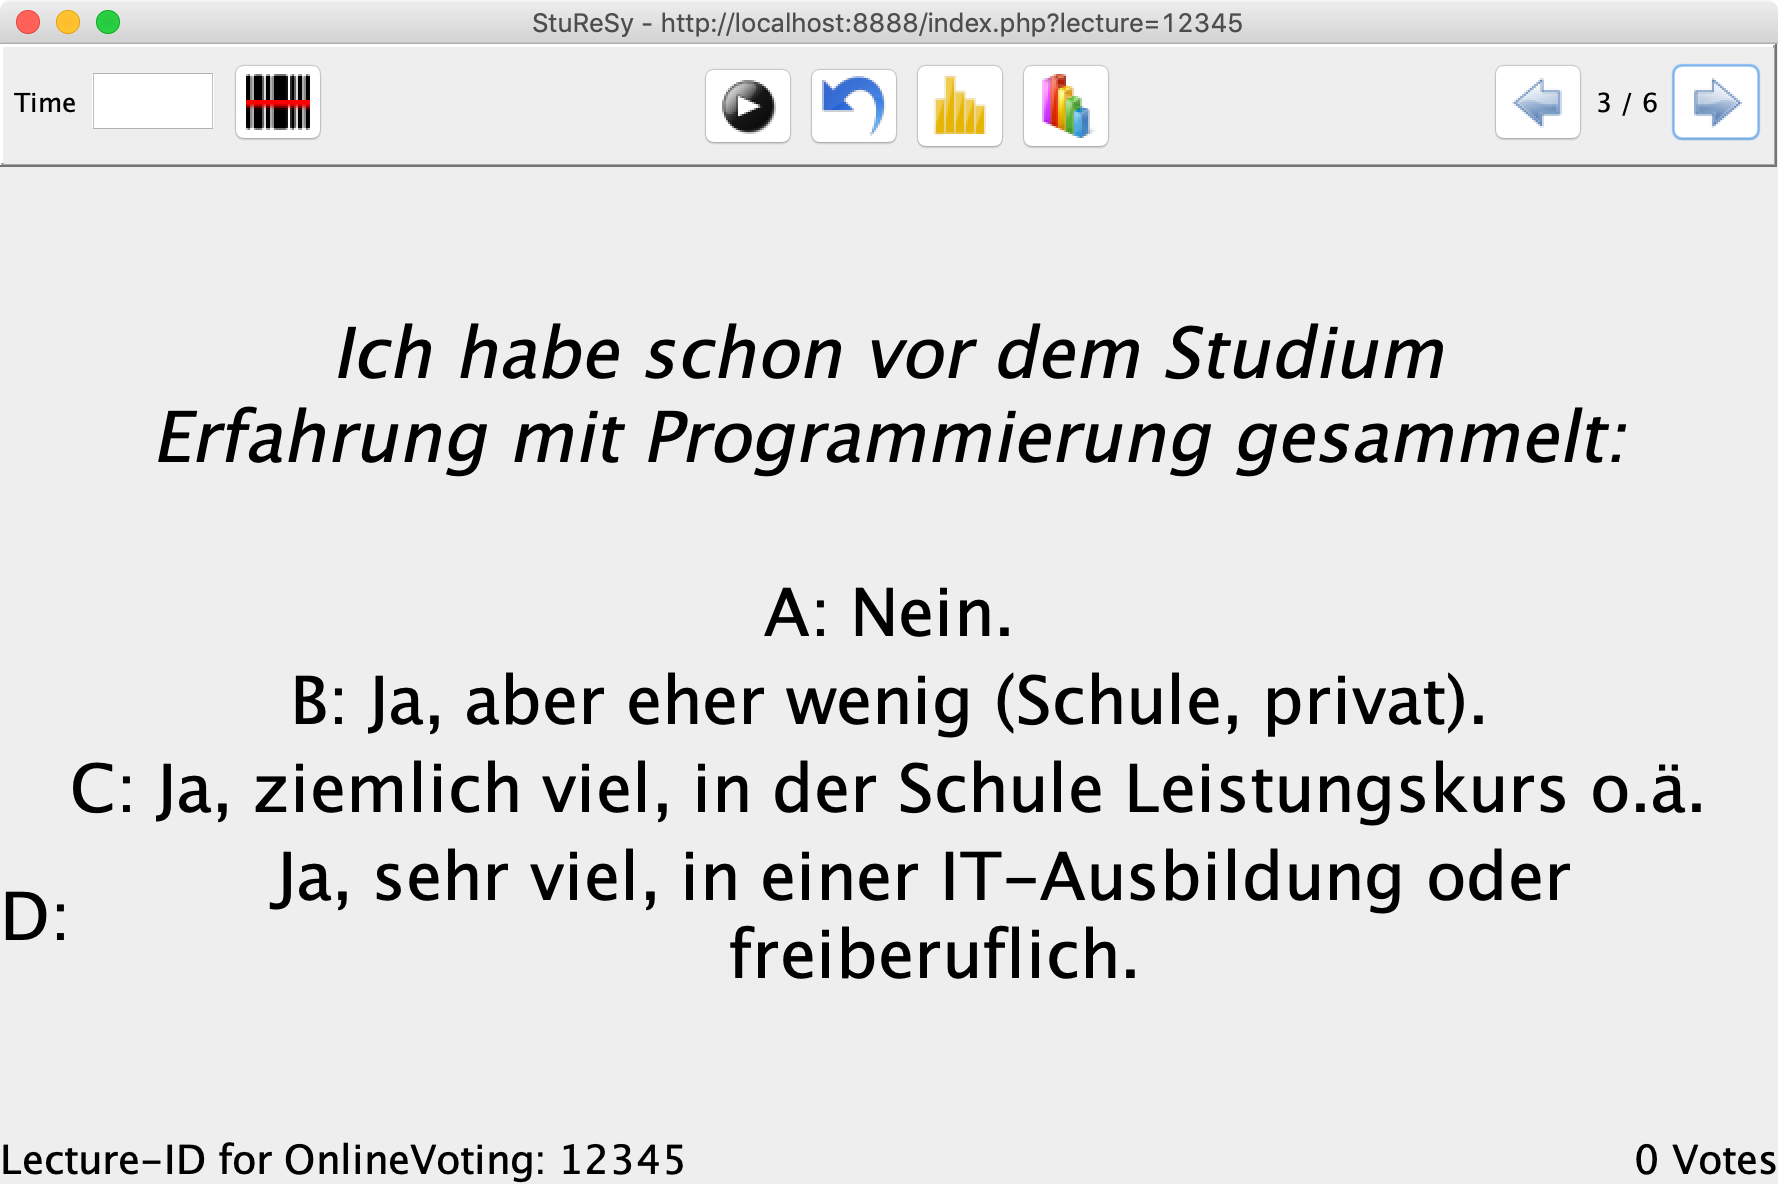
\includegraphics[width=11cm]{chapter/bewertung/bilder/StuReSy_Problem_1.png}
    \centering
    \caption{Die horizontale und vertikale Ausrichtung der Antwort-Möglichkeiten ist unregelmäßig und erschwert die optische Zuordnung der einzelnen Zeilen.}
    \label{abb:sturesy_problem_2}
\end{figure}

\begin{figure}[H]
    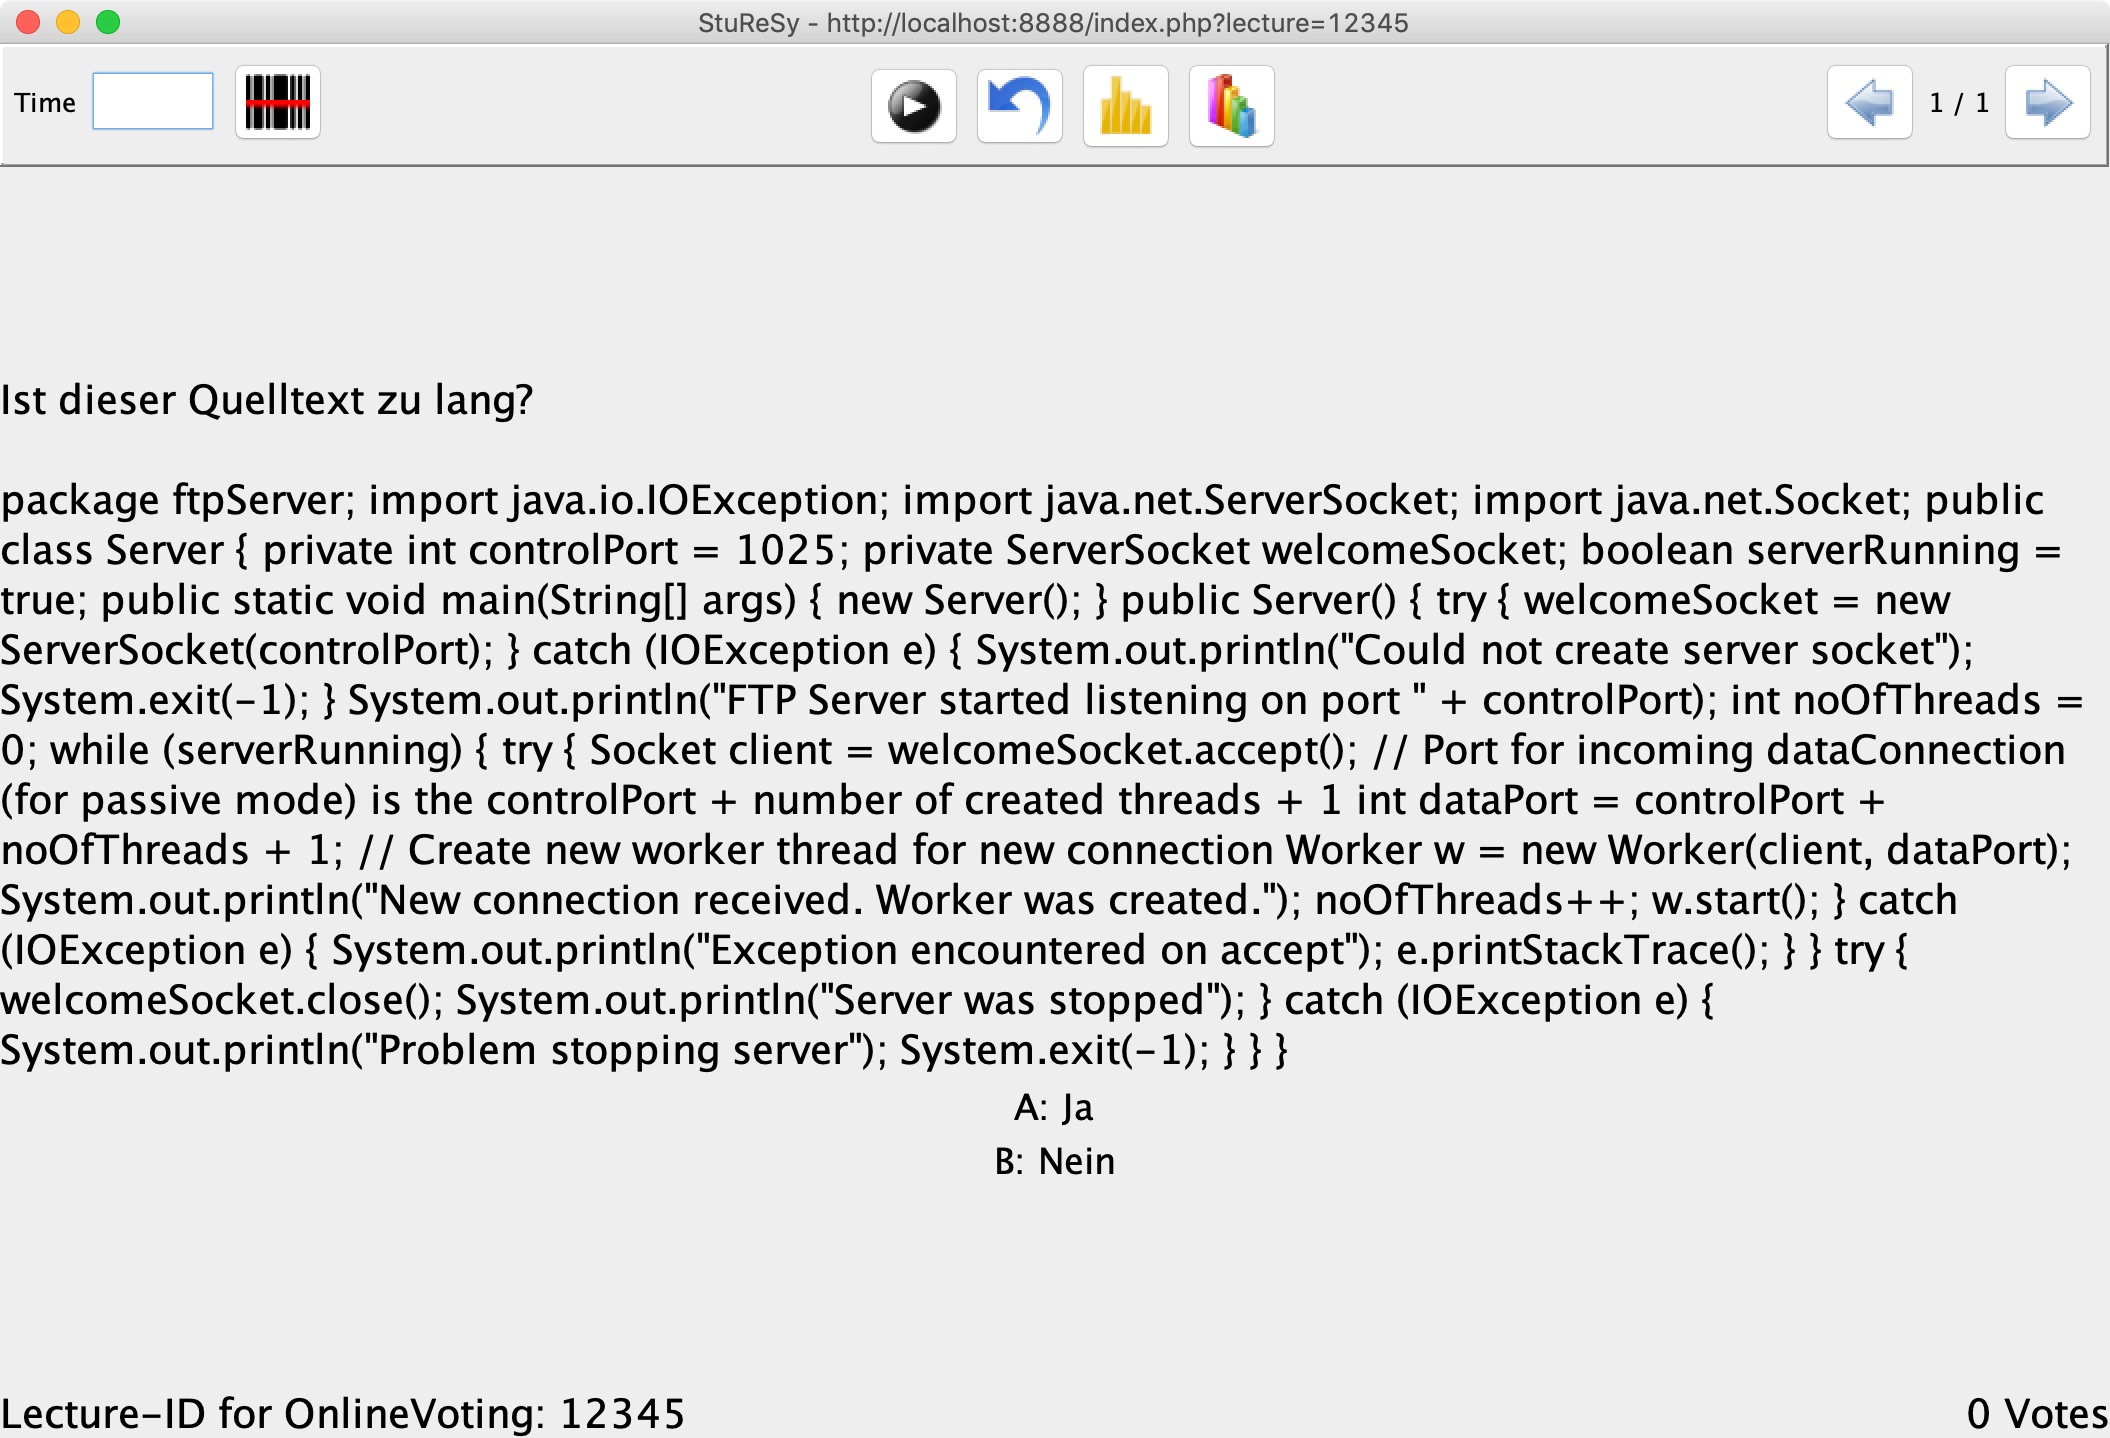
\includegraphics[width=11cm]{chapter/bewertung/bilder/StuReSy_Problem_3.png}
    \centering
    \caption{Beim Einfügen von Quelltexten aus der Zwischenablage, gehen sämtliche Whitespace-Formatierungen verloren und müssen manuell wieder eingefügt werden.}
    \label{abb:sturesy_problem_3}
\end{figure}
